\documentclass[letterpaper,addpoints,answers]{exam}
\usepackage{graphicx}
\usepackage{multicol}
\usepackage{wrapfig}
\usepackage{tikz}

\usetikzlibrary{calc}

\makeatletter
\def\grd@save@target#1{%
  \def\grd@target{#1}}
\def\grd@save@start#1{%
  \def\grd@start{#1}}
\tikzset{
  grid with coordinates/.style={
    to path={%
      \pgfextra{%
        \edef\grd@@target{(\tikztotarget)}%
        \tikz@scan@one@point\grd@save@target\grd@@target\relax
        \edef\grd@@start{(\tikztostart)}%
        \tikz@scan@one@point\grd@save@start\grd@@start\relax
        \draw[minor help lines] (\tikztostart) grid (\tikztotarget);
        \draw[major help lines] (\tikztostart) grid (\tikztotarget);
        \grd@start
        \pgfmathsetmacro{\grd@xa}{\the\pgf@x/1cm}
        \pgfmathsetmacro{\grd@ya}{\the\pgf@y/1cm}
        \grd@target
        \pgfmathsetmacro{\grd@xb}{\the\pgf@x/1cm}
        \pgfmathsetmacro{\grd@yb}{\the\pgf@y/1cm}
        \pgfmathsetmacro{\grd@xc}{\grd@xa + \pgfkeysvalueof{/tikz/grid with coordinates/major step x}}
        \pgfmathsetmacro{\grd@yc}{\grd@ya + \pgfkeysvalueof{/tikz/grid with coordinates/major step y}}
        \foreach \x in {\grd@xa,\grd@xc,...,\grd@xb}
        \node[anchor=north] at (\x,\grd@ya) {\pgfmathprintnumber{\x}};
        \foreach \y in {\grd@ya,\grd@yc,...,\grd@yb}
        \node[anchor=east] at (\grd@xa,\y) {\pgfmathprintnumber{\y}};
      }
    }
  },
  minor help lines/.style={
    help lines,
    gray,
    line cap =round,
    xstep=\pgfkeysvalueof{/tikz/grid with coordinates/minor step x},
    ystep=\pgfkeysvalueof{/tikz/grid with coordinates/minor step y}
  },
  major help lines/.style={
    help lines,
    line cap =round,
    line width=\pgfkeysvalueof{/tikz/grid with coordinates/major line width},
    xstep=\pgfkeysvalueof{/tikz/grid with coordinates/major step x},
    ystep=\pgfkeysvalueof{/tikz/grid with coordinates/major step y}
  },
  grid with coordinates/.cd,
  minor step x/.initial=.5,
  minor step y/.initial=.2,
  major step x/.initial=1,
  major step y/.initial=1,
  major line width/.initial=1pt,
}
\makeatother

\tikzset{
    right angle quadrant/.code={
        \pgfmathsetmacro\quadranta{{1,1,-1,-1}[#1-1]}     % Arrays for selecting quadrant
        \pgfmathsetmacro\quadrantb{{1,-1,-1,1}[#1-1]}},
    right angle quadrant=1, % Make sure it is set, even if not called explicitly
    right angle length/.code={\def\rightanglelength{#1}},   % Length of symbol
    right angle length=2ex, % Make sure it is set...
    right angle symbol/.style n args={3}{
        insert path={
            let \p0 = ($(#1)!(#3)!(#2)$) in     % Intersection
                let \p1 = ($(\p0)!\quadranta*\rightanglelength!(#3)$), % Point on base line
                \p2 = ($(\p0)!\quadrantb*\rightanglelength!(#2)$) in % Point on perpendicular line
                let \p3 = ($(\p1)+(\p2)-(\p0)$) in  % Corner point of symbol
            (\p1) -- (\p3) -- (\p2)
        }
    }
}

\begin{document}

\begin{coverpages}
 \large\bfseries
 
 \noindent 
 Physics 107: Physics for Life-Sciences

 \vspace{2ex}
 \noindent
 Midterm Exam: September 21, 2015

 \vspace{3ex}
 \noindent 
 This test is administered under the rules and regulations of the honor code of the College of William \& Mary.

 \vspace{2ex}
 \noindent 
 Name:\enspace\makebox[2.3in]{\hrulefill} \\

 \noindent 
 Signature:\enspace\makebox[2in]{\hrulefill} \\

 \vspace{5ex}
 \noindent 
 Instructions:
 \begin{itemize}
  \item This is a closed book, closed notes test.
  \item Calculators are NOT needed and NOT allowed. Devices with wireless connections are NOT allowed.
  \item Start your work from the fundamental equations on the formula sheet, and derive any additional expressions that you may need.
  \item Circle your answer for each part of each problem. 
  \item Clearly mark out any work that you wish the grader to disregard.  Do not waste your time erasing.
  \item Your work will be graded based on your ability to write down a logical and organized solution grounded in the correct assessment of the physics of a situation. No credit will be given for an answer that is not justified by a logical solution or where that justification is not organized or readable. Partial credit will be given up to the point where your solution departs from a correct analysis of the physics involved for any given part of a problem.
 \end{itemize}

 \pagebreak

 \begin{center}
  \gradetable[v][questions]
 \end{center}
 
\end{coverpages}
 

\begin{questions}

\printanswers

\question[5]
You are operating a small remote controlled toy car on the sidewalk along Jamestown Road. As you are standing on the sidewalk, the speed of the toy car relative to you is plotted below.  What is the displacement of the toy car between 0\,s and 13\,s?

\begin{center}
 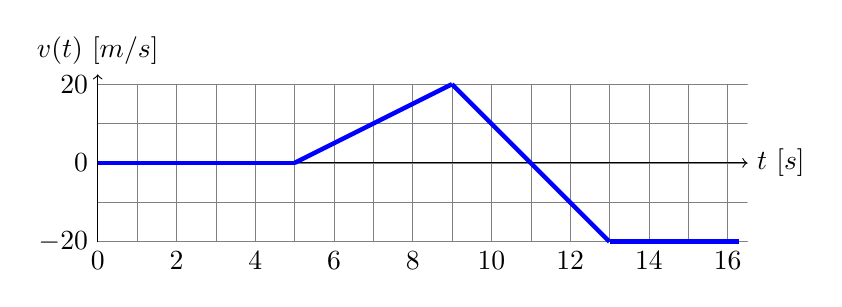
\begin{tikzpicture}[xscale=0.5,yscale=0.05,grid with coordinates/major step x=2,grid with coordinates/minor step x=1,grid with coordinates/major step y=20,grid with coordinates/minor step y=10,grid with coordinates/major line width=0.2pt]
  \draw (0,-20) to[grid with coordinates] (16.5,20);
  \draw[->] (0,0) -- (16.5,0) node[right] {$t~[s]$};
  \draw[->] (0,-20) -- (0,22.5) node[above] {$v(t)~[m/s]$};
  \draw[ultra thick,color=blue] (0.0,0.0) -- (5.0,0.0);
  \draw[ultra thick,color=blue] (5.0,0.0) -- (9.0,+20.0);
  \draw[ultra thick,color=blue] (9.0,+20.0) -- (13.0,-20.0);
  \draw[ultra thick,color=blue] (13.0,-20.0) -- (16.3,-20.0);
 \end{tikzpicture}
\end{center}
\begin{checkboxes}
 \choice -20\,m
 \choice 4\,m
 \correctchoice 40\,m
 \choice 80\,m
 \choice 300\,m
\end{checkboxes}

\question[5]
The graph below shows position as a function of time for two trains on parallel tracks. Which of the statements is true?
\begin{center}
 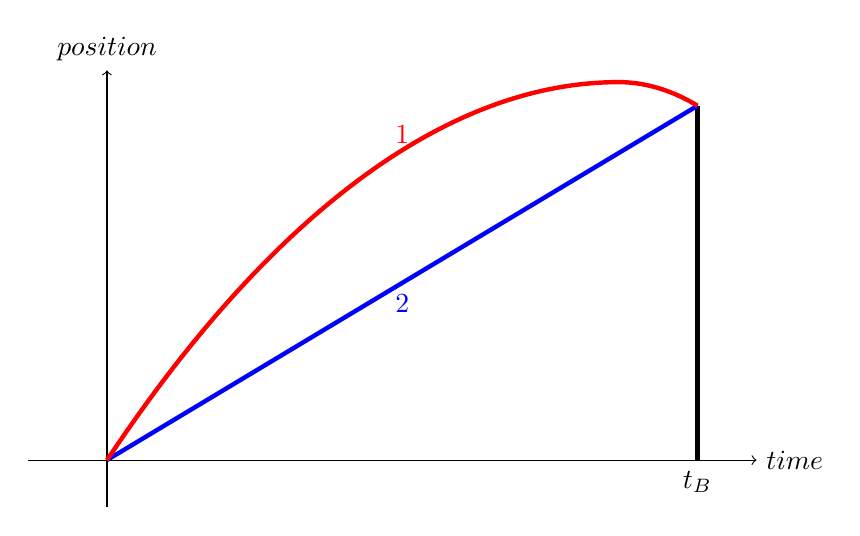
\begin{tikzpicture}[xscale=0.5,yscale=0.3,grid with coordinates/major step x=2,grid with coordinates/minor step x=1,grid with coordinates/major step y=20,grid with coordinates/minor step y=10,grid with coordinates/major line width=0.2pt]
  \draw[->] (-2,0) -- (16.5,0) node[right] {$time$};
  \draw[->] (0,-2) -- (0,16.5) node[above] {$position$};
  \draw[ultra thick] (15.0,0.0) node[below,color=black]{$t_B$} -- (15.0,15.0);
  \draw[ultra thick,color=blue] (0.0,0.0) -- node[below]{$2$} (15.0,15.0);
  \draw[ultra thick,color=red] (15.0,15.0) parabola bend (13.0,16.0) (0.0,0.0);
  \draw (7.5,13.0) node[above,color=red]{$1$};
 \end{tikzpicture}
\end{center}
\begin{checkboxes}
 \choice Train $1$ has a larger displacement than train $2$ between time $0$ and $t_B$.
 \choice At time $t_B$, both trains have the same velocity.
 \choice Both trains speed up all the time.
 \correctchoice Both trains have the same velocity at some time before $t_B$.
 \choice Somewhere on the graph, both trains have the same acceleration.
\end{checkboxes}

\question[5]
A ball is thrown straight up, reaches a maximum height, and then falls back downward. Which of the following are true when it reaches its maximum height?
\begin{checkboxes}
 \choice Its velocity and its acceleration are zero.
 \choice Its velocity is zero and its acceleration points upward.
 \correctchoice Its velocity is zero and its acceleration points downward.
 \choice Its velocity points downward and its acceleration points upward.
 \choice Its velocity and its acceleration point downward.
\end{checkboxes}

\pagebreak

\begin{multicols}{2}
\question
A waiter is serving drinks at a seafood restaurant and carrying a tray with a mass $m_1 = 0.500$\,kg. On top of the tray are a bottle and some glasses with a total mass $m_2 = 2.000$\,kg. The waiter pushes up from below with a force $\vec{F}$ with a magnitude of 30.0\,N. You can approximate the gravitational acceleration as $g \approx 10$\,m/s$^2$. You may consider the bottle and glasses as a single object.
\columnbreak
\begin{center}
 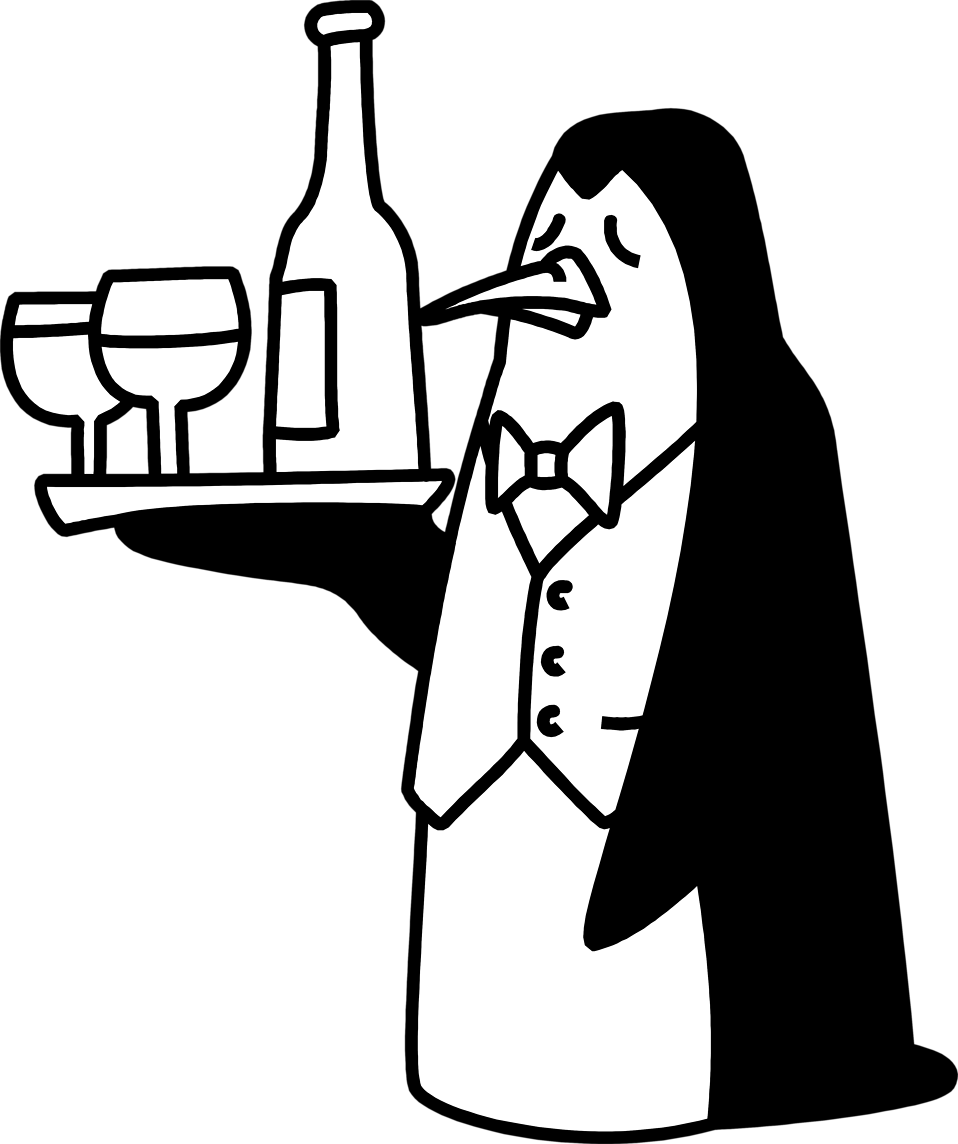
\includegraphics[width=10em]{test1/illustration-of-a-penguin-waiter-serving-drinks-on-a-tray}
\end{center}
\end{multicols}
\begin{parts}
\part[5] What is the acceleration (nagnitude and direction) of the entire tray and its contents?
\begin{solution}[2in]
The total mass of the entire tray and its contents is $m = m_1 + m_2 = 2.500$\,kg. The weight of this total mass is $\vec{W} = m \vec{g} = 25$\,N downwards. The net force $\vec{F}_{net} = \vec{F} + \vec{W}$ is then 5\,N upwards. The acceleration that results from this net force $\vec{F}_{net}$ is then $\frac{F_{net}}{m} = 2.0$\,m/s upwards.
\end{solution}
\part[10] What is the force (magnitude and direction) that the tray exerts on the bottle and glasses?
\begin{solution}[2in]
Since the bottle and glasses with mass $m_2$ are moving upwards with an acceleration of 2.0\,m/s, the net force on the bottle and glasses must be $m_2 a = 4.0$\,N upwards. Since the weight on the bottle and glasses is $\vec{W}_2 = \vec{m}_2 g = 20$\,N downwards, this means that the force from the tray on the bottle and glasses is 24\,N upwards. 
\end{solution}
\part[5] What is the force (magnitude and direction) that the bottle and glasses exert on the tray?
\begin{solution}
The force of the bottle and glasses on the tray is equal and opposite to the force of the tray on the bottle and glasses due to Newton's third law, and therefore 24\,N downwards.
\end{solution}
\end{parts}

\pagebreak

\question
\begin{multicols}{2}
Chessie is a legendary sea monster said to live in the midst of the Chesapeake Bay. Chessie starts swimming from the Gloucester Point marina and wants to reach Yorktown on the other shore of the York river, directly to the southwest of Gloucester Point. Chessie can swim with a speed of 10.0\,knots (or 10.0 nautical miles per hour) relative to the water. However, the tide is coming in from the Chesapeake Bay and there is a current from the southeast to the northwest with a speed of 8.0\,knots relative to the ground.
\columnbreak
\begin{flushright}
 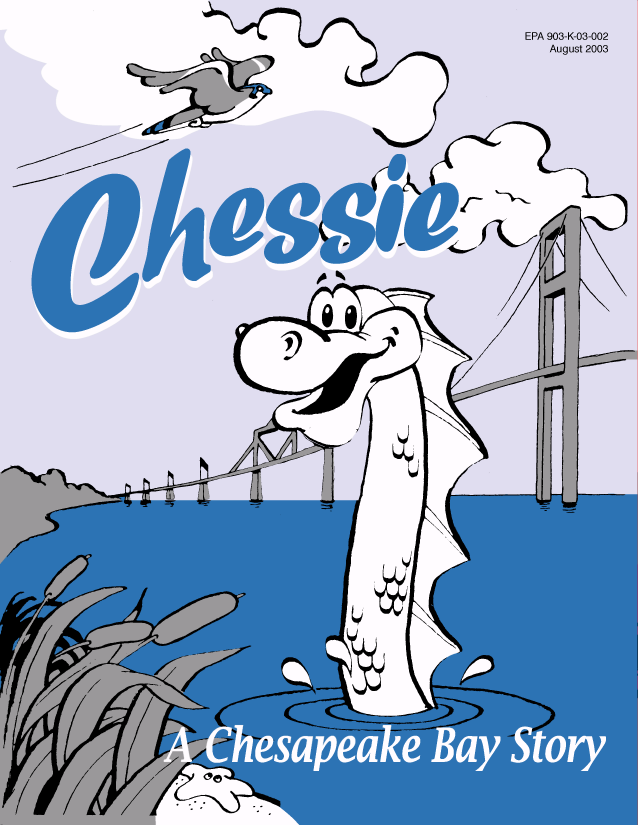
\includegraphics[width=12em]{test1/Chessie_A_Chesapeake_Bay_Story_Cover_Art}
\end{flushright}
\end{multicols}
\begin{parts}
\part[5] In approximately which of the four cardinal directions with respect to the water must Chessie swim to reach Yorktown?
\begin{solution}[2in]
We start from the relative velocity expression $\vec{v}_{chessie,ground} = \vec{v}_{chessie,water} + \vec{v}_{water,ground}$. Since $\vec{v}_{chessie,ground}$ should be towards the southwest and $\vec{v}_{water,ground}$ is towards the northwest, Chessie will have to swim approximately towards the south.
\end{solution}
\part[10] The distance between the Gloucester Point marina and Yorktown is exactly 2.0 nautical miles. How long does it take Chessie to reach Yorktown?
\begin{solution}[2in]
We start from the relative velocity expression $\vec{v}_{chessie,ground} = \vec{v}_{chessie,water} + \vec{v}_{water,ground}$. We know $|\vec{v}_{chessie,water}| = 10.0$\,knots, $\vec{v}_{water,ground} = 8.0$\,knots to the northwest, and $\vec{v}_{chessie,ground}$ is in the direction southwest. In the vector addition we have a right angle between $\vec{v}_{chessie,ground}$ (southwest) and $\vec{v}_{water,ground}$ (northwest) so we can use the Pythagorean theorem, $|\vec{v}_{chessie,ground}|^2 + |\vec{v}_{water,ground}|^2 = |\vec{v}_{chessie,water}|^2$, to determine $|\vec{v}_{chessie,ground}| = \sqrt{10.0^2 - 8.0^2} = 6.0$\,knots. At a speed of 6.0 nautical miles per hour, it takes Chessie 20 minutes to reach the other shore.
\begin{center}
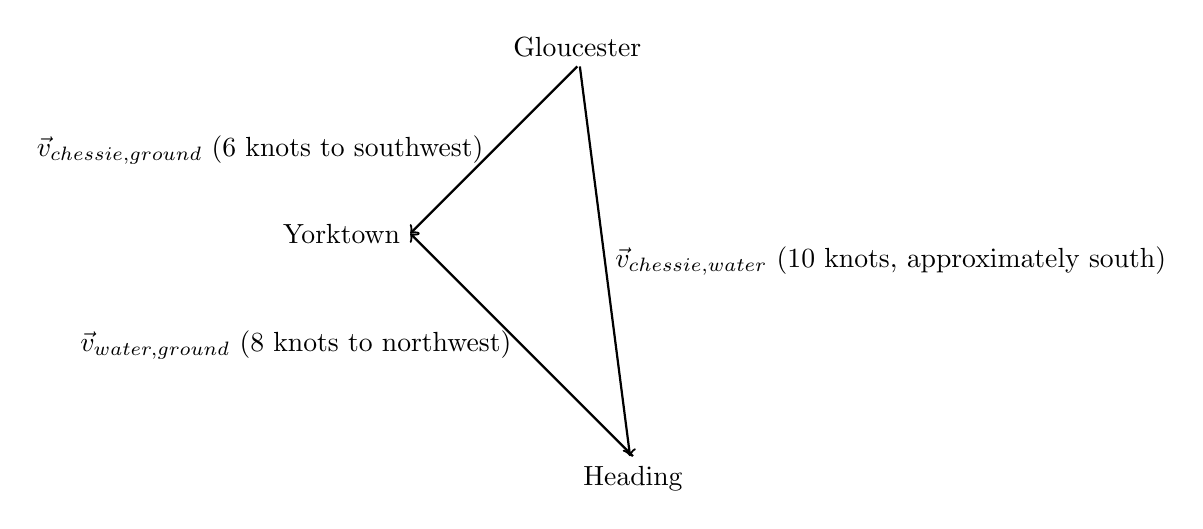
\begin{tikzpicture}[xscale=0.5,yscale=0.5]
\draw[thick,<-] (0,0) node[left]{Yorktown} -- node[midway,left]{$\vec{v}_{chessie,ground}$ (6 knots to southwest)} ++(45:6) node[above](gloucester){Gloucester};
\draw[thick,<-] (0,0) -- node[midway,left]{$\vec{v}_{water,ground}$ (8 knots to northwest)} ++(-45:8) node[below](heading){Heading};
\draw[thick,->] (gloucester) -- node[midway,right]{$\vec{v}_{chessie,water}$ (10 knots, approximately south)} (heading);
\end{tikzpicture}
\end{center}
\end{solution}
\end{parts}

\pagebreak

\question
Physics departments often have a Halloween \emph{pumpkin drop}. In this event, physics students drop pumpkins from the roof of their building with a height of 16.0\,m. A student throws a pumpkin with a initial speed of 4.0 m/s at an angle of $60^\circ$ from the vertical. You can approximate the gravitational acceleration as $g \approx 10$\,m/s$^2$.

\begin{parts}
\part[5] What is the maximum height above the ground that the pumpkin reaches before it falls to the ground?
\begin{solution}[1.5in]
We can use the formula $h = y_0 + \frac{v_0^2}{2 g} \sin^2 \theta$ to determine the height the pumpkin will reach when its starting position is $y_0 = 18.0$\,m. In particular, with $\theta = 30^\circ$ the angle with the horizontal, this gives us a maximum height of 18.2\,m.
\end{solution}
\part[5] What is the vertical component of the initial velocity?
\begin{solution}[1.5in]
The angle $\theta = 30^\circ$ is angle with the horizontal, so the vertical component of the initial velocity is $v_{0,y} = v_0 \sin 30^\circ = +2.0$\,m/s.
\end{solution}
\part[5] How long does it take for the pumpkin to reach the ground, starting from the time it is released? You may find the following useful: $10^2 = 100$, $11^2 = 121$, $12^2 = 144$, $13^2 = 169$, $14^2 = 196$, $15^2 = 225$, $16^2 = 256$, $17^2 = 289$, $18^2 = 324$, $19^2 = 361$, $20^2 = 400$.
\begin{solution}[2in]
We start from the vertical motion equation $y = y_0 + v_{0,y} t - \frac{1}{2} g t^2$ where $y = 0$, $y_0 = 18.0$\,m, and $v_{0,y} = 2.0$\,m/s. The equation to solve is then $0 = 16.0\,\hbox{m} + 2.0\,\hbox{m/s}\cdot t - 5\,\hbox{m/s}^2 \cdot t^2$. The solutions to this quadratic equation are $t = \frac{2 \pm 18}{10}$ of which we are interested in the positive solution $t = 2.0$\,s.
\end{solution}
\part[5] What is the vertical component of the velocity on impact?
\begin{solution}[1.5in]
After a time $t = 2.0$\,s the velocity has changed from $v_{0,y} = +2.0$\,m/s to $v_y = v_{0,y} - g t = -18.0$\,m/s. This could have been obtained directly from $v_y^2 = v_{0,y}^2 - 2 g (y - y_0) = 4\,\hbox{m}^2/\hbox{s}^2 - 20\,\hbox{m}/\hbox{s}^2 (-16\,\hbox{m}) = 324\,\hbox{m}^2/\hbox{s}^2$.
\end{solution}
\end{parts}


\end{questions}

 \pagebreak
 
 {\Large Possibly useful relations (feel free to detach this page):}
  
 \fontseries{\seriesdefault}
 \begin{multicols}{2}
 \Large
 \noindent
 $\vec{v}_{avg} = \Delta\vec{x} / \Delta t$ \\
 $x = x_0 + v_0 t + \frac{1}{2} a t^2$ \\
 $v^2 = v_0^2 + 2 a (x - x_0)$ \\
 $R = \frac{v_0^2}{g}\sin 2\theta$ \\
 $\vec{F}_{net} = m \vec{a}$ \\
 $\vec{W} = m \vec{g}$ \\
 $\cos\theta = \hbox{adjacent}/\hbox{hypotenuse}$ \\
 $\sin\theta = \hbox{opposite}/\hbox{hypotenuse}$ \\
 $\sin 30^\circ = \cos 60^\circ = \frac{1}{2}$ \\
 $\cos 30^\circ = \sin 60^\circ = \frac{\sqrt{3}}{2}$ \\
 
 \noindent
 $\vec{a}_{avg} = \Delta\vec{v} / \Delta t$ \\
 $v = v_0 + a t$ \\
 $v_{avg} = \frac{v_0 + v}{2}$ \\
 $h = \frac{v_0^2}{2 g} \sin^2 \theta$ \\
 $\vec{F}_{BA} = - \vec{F}_{AB}$ \\
 $\vec{g} = 9.80\,m/s^2$ downward \\
 $x = \frac{-b \pm \sqrt{b^2 - 4 a c}}{2 a}$ \\
 $\tan\theta = \sin\theta / \cos\theta$ \\
 $\tan 45^\circ = 1$ \\
 \end{multicols}

\end{document}
